\subsection{Robustheit gegenüber Lichtverhältnissen}
\label{sec:brightness_eval}
\begin{figure}[h!]
    \centering
    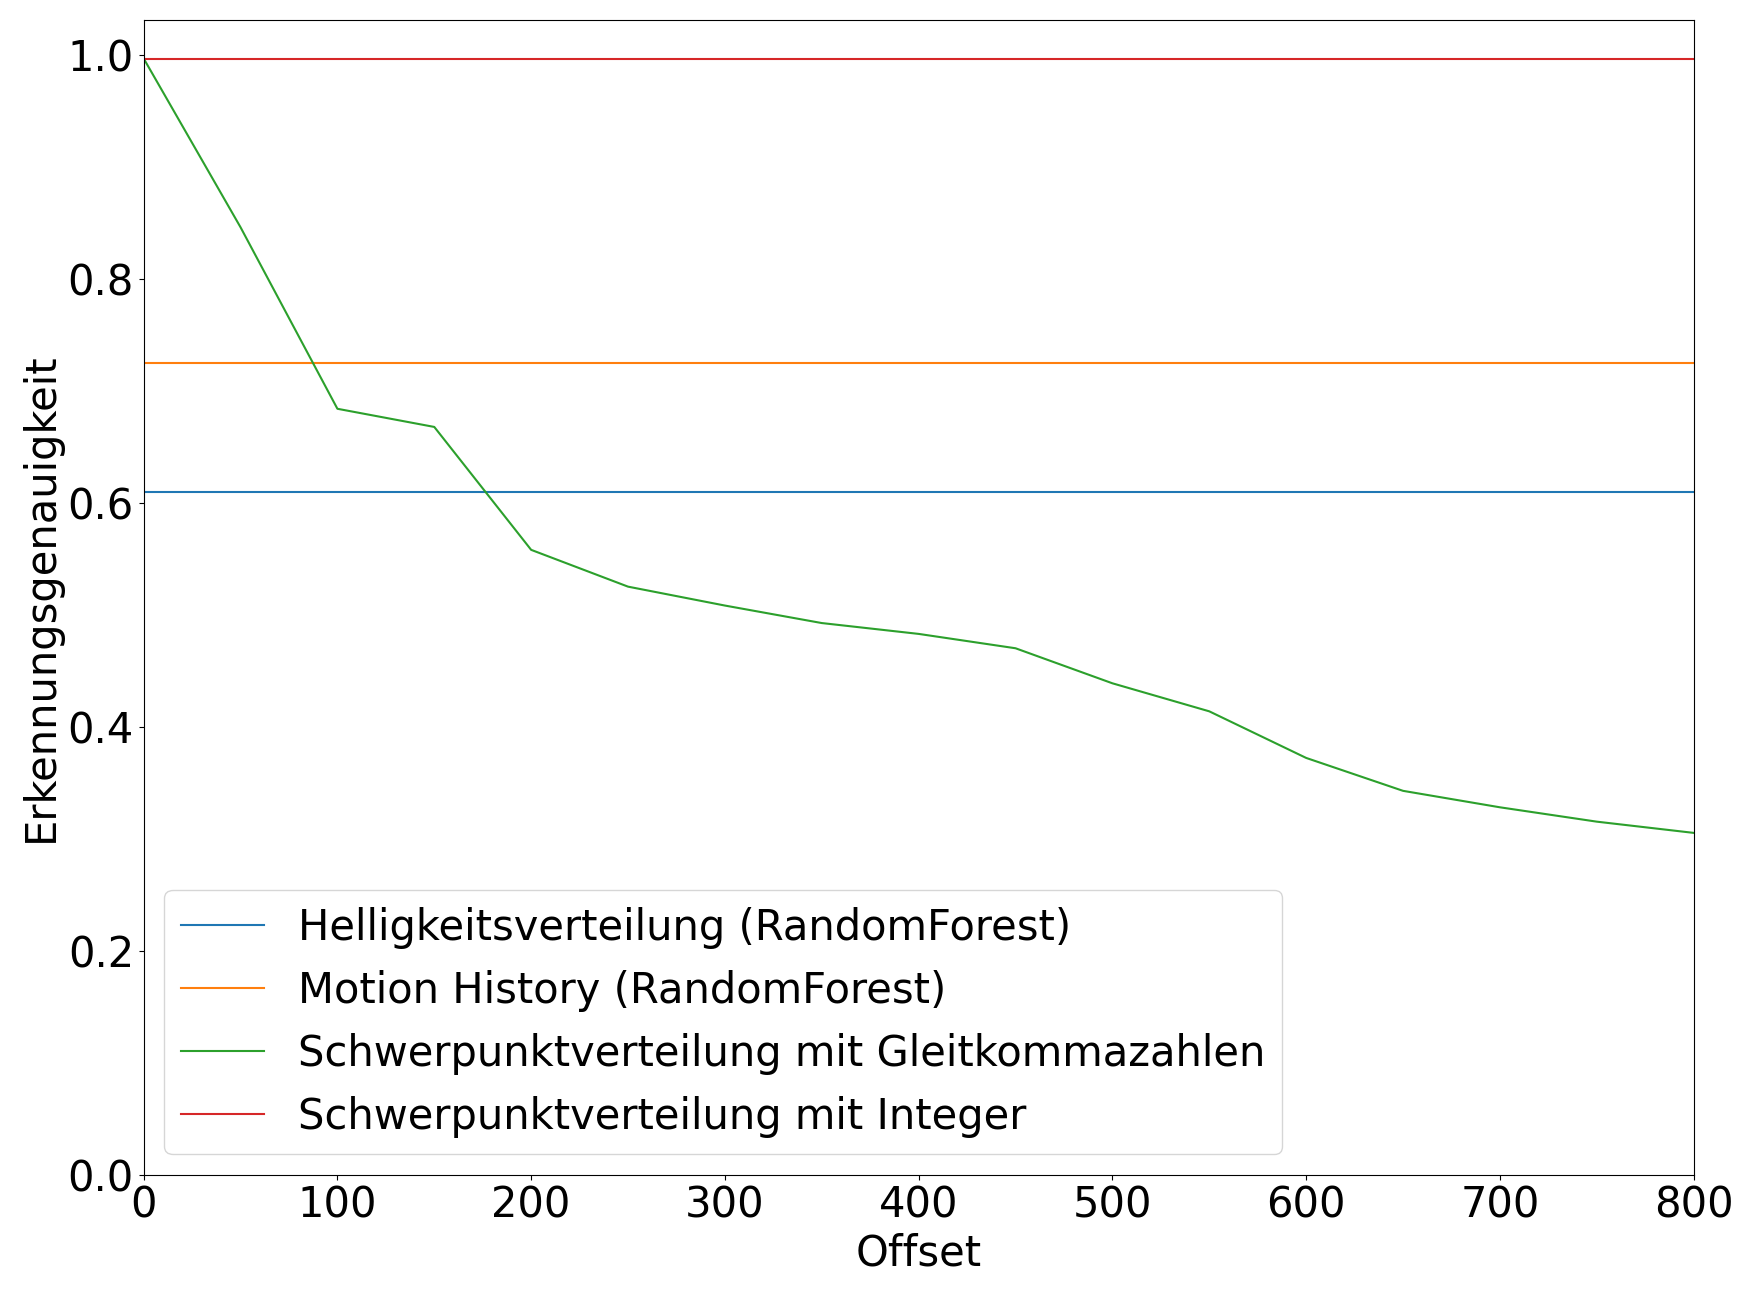
\includegraphics[width=\linewidth]{images/brightness_offset.png}
    \caption{Ergebnisse des Offset der Helligkeitstestmenge 1 je Ansatz.}
    \label{fig:brightness_offset}
\end{figure}
Dieses Kapitel validiert die Invarianzen der einzelnen Features, die in Kapitel \ref{sec:feature_selection} diskutiert wurden. Mit Hilfe der Helligkeitstestmengen werden die Features validiert. Diese synthetischen Testmengen
verändern die Helligkeit und den Kontrast einer bestehenden Testmenge durch Skalierung und Offsets.
\newline
\newline
Abbildung \ref{fig:brightness_offset} zeigt, wie sich ein zunehmender Offset zwischen 0 und 800 auf die Klassifizierer auswirkt. Dabei erhöht sich die Gesamthelligkeit, aber der Kontrast bleibt gleich.
Die Helligkeitsverteilung, Motion History und Schwerpunktverteilung mit Ganzzahlen bleiben
konstant. Daher wird geschlossen, dass diese invariant gegenüber einem Offset sind. Die kombinierte Schwerpunktverteilung ist sehr robust gegenüber einen Offset aber nicht invariant. Bei einem Offset zwischen 300
und 500 ist der stärkste Einbruch der Klassifizierungsgenauigkeit zu beobachten. Das ist auf die Schwerpunktverteilung mit Gleitkommazahlen zurückzuführen, die massive Einbrüche der Klassifizierungsgenauigkeit
mit zunehmendem Offset erfährt. Zwischen 300 und 500 ist der Einbruch am größten. Die Schwerpunktverteilung mit Gleitkommazahlen ist sehr anfällig gegenüber einem Offset.
\begin{figure}[h!]
    \centering
    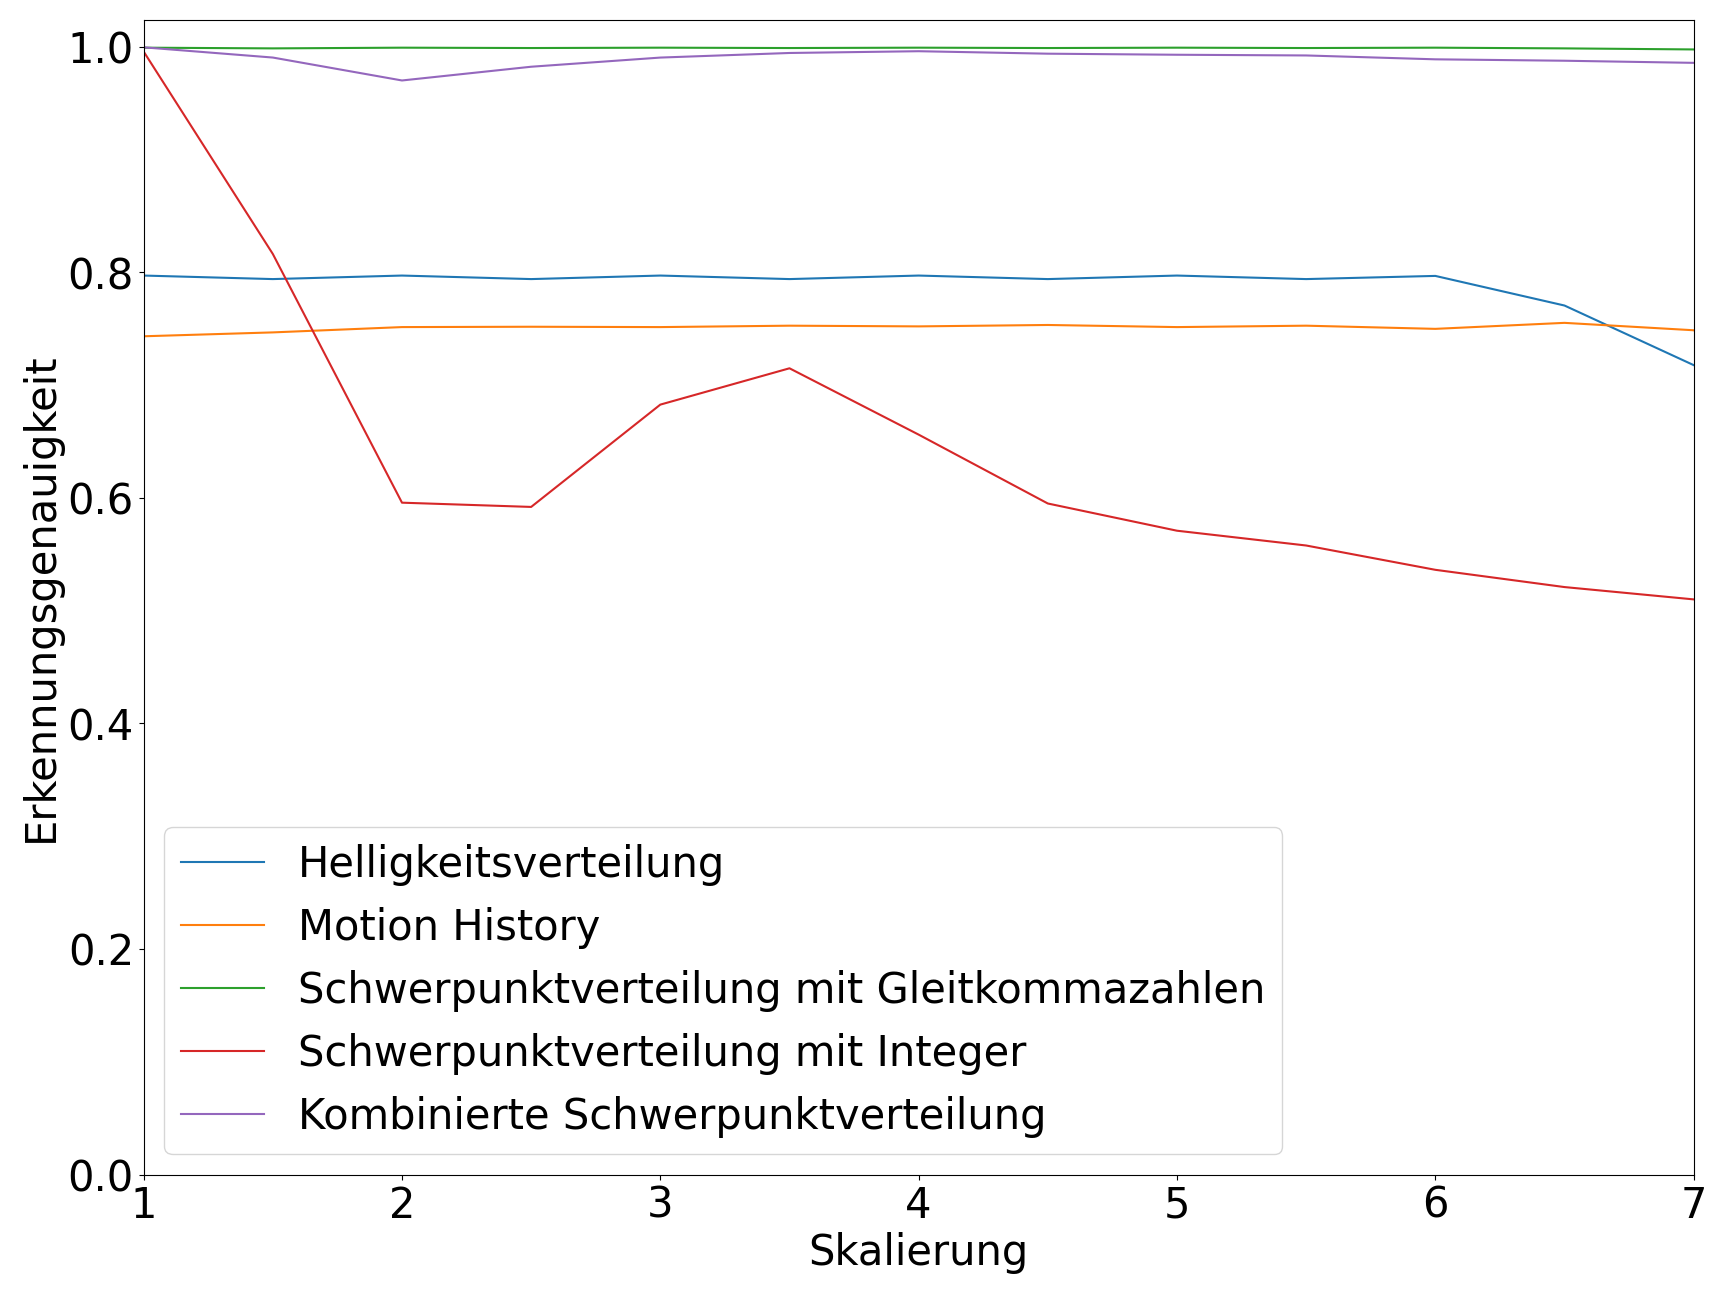
\includegraphics[width=\linewidth]{images/brightness_scaling.png}
    \caption{Ergebnisse der Skalierung der Helligkeitstestmenge 1 je Ansatz.}
    \label{fig:brightness_scaling}
\end{figure}
\newline
\newline
Abbildung \ref{fig:brightness_scaling} zeigt, wie sich ein zunehmender Skalierungsfaktor auf die Klassifizierer auswirkt. Dabei erhöht sich sowohl die Gesamthelligkeit, als auch der Kontrast. Die Schwerpunktverteilung mit
Gleitkommazahlen, die Helligkeitsverteilung und die Motion History zeigen eine Invarianz gegenüber Skalierung. Ab einem Faktor von 6,5 und 7 sind Einbrüche zu erkennen. Die Trainingsmenge, auf der die
Helligkeitstestmenge 1 basiert, enthält aber auch Einträge mit Helligkeiten oberhalb 160, sodass eine Skalierung mit 6,5 Clipping-Effekte erzeugt, d. h. Pixel mit einer Helligkeit
über 1023 werden auf 1023 gesetzt. Die Schwerpunktverteilung mit Ganzzahlen erfährt starke Einbrüche in der Klassifizierungsgenauigkeit, ähnlich wie die Schwerpunktverteilung mit Gleitkommazahlen im
Vergleich zum Offset. Allerdings ist der maximale Einbruch der Klassifizierungsgenauigkeit geringer. Sie ist aber trotzdem sehr anfällig gegenüber der Skalierung. Die kombinierte Schwerpunktverteilung
ist sehr robust gegenüber der Skalierung aber nicht invariant. Sie weist ebenfalls Einbrüche der Klassifizierungsgenauigkeit zwischen 6,5 und 7 auf aber auch zwischen 1,5 und 3,5. Dies ist
auf die Schwerpunktverteilung mit Ganzzahlen zurückzuführen.
\begin{figure}[h!]
    \centering
    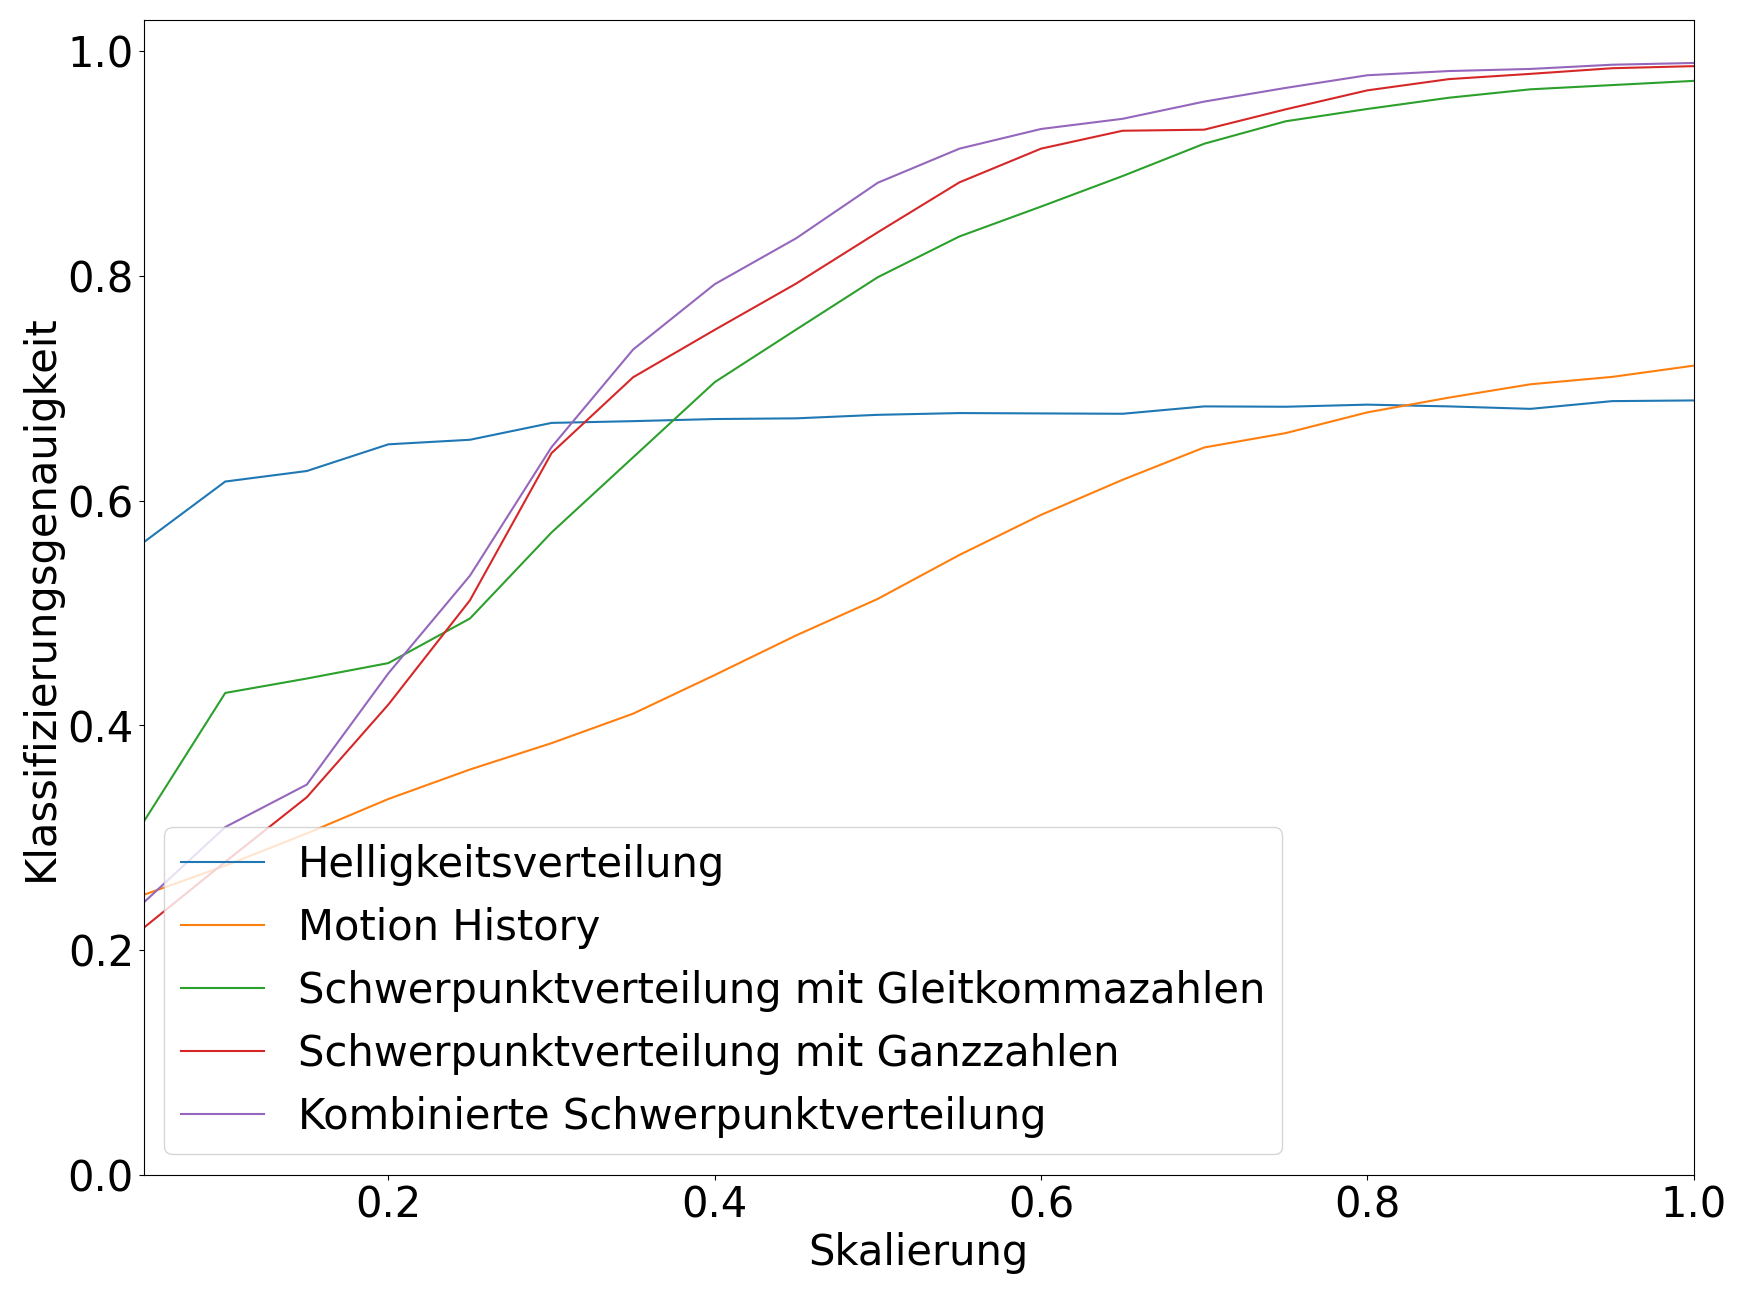
\includegraphics[width=\linewidth]{images/brightness2_scaling.png}
    \caption{Ergebnisse der Helligkeitstestmenge 2 je Ansatz.}
    \label{fig:brightness2_scaling}
\end{figure}
\newline
\newline
Abbildung \ref{fig:brightness2_scaling} zeigt, wie sich sich ein abnehmender Kontrast bei gleichbleibender Helligkeit auf die Klassifizierer auswirkt. Diese Situation ist vergleichbar mit einer zunehemden Distanz
zur Kamera, da dort der Kontrast durch Streulicht ebenfalls geringer wird. Keiner der Feature-Mengen weist eine Invarianz dem gegenüber auf. Die Helligkeitsverteilung ist bis zu einem Faktor von 0,3 sehr stabil. Ab 0,3
nimmt die Klassifizierungsgenauigkeit leicht ab. Bei einem initialen Kontrastunterschied von 100\% ist ab 0,3 der Kontrast nur noch 18\% des ursprünglichen Kontrasts. Dementsprechend ist die Helligkeitsverteilung extrem
robust gegenüber schlechten Lichtverhältnissen. Im Vergleich sind die anderen Klassifizierer sehr sensibel gegenüber der abnehmenden Skalierung bei gleichbleibender Gesamthelligkeit.
\newpage
Die Schwerpunktverteilungen verhalten sich vom Trend her gleich, aber die
kombinierte Schwerpunktverteilung erzielt wie erwartet, fast durchweg, die beste Klassifizierungsgenauigkeit. Da keiner der Schwerpunktverteilungen invariant gegenüber einem Offset und der Skalierung waren, war auch
nicht zu erwarten, dass sie eine Invarianz in diesem Test zeigen. Trotzdem erzielen sie die beste Klassifizierungsgenauigkeit bis zu einem Faktor von 0,3. Von der Motion History war ein ähnliches Verhalten wie bei der
Helligkeitsverteilung zu erwarten. Vermutet wird, dass die unterliegende Funktion, um eine Bewegung zu detektieren, zu restriktiv wird, wenn der Kontrast sinkt.
\newline
\newline
Kubik hat beobachtet, dass bei zunehmender Distanz der Kontrast geringer wird. Seine KNN haben mit abnehmenden Kontrast geringere Klassifizierungsgenauigkeiten erzielt \cite{kubikThesis}. Dieses Verhalten wird durch die
Helligkeitstestmenge 2 bestätigt. Erstaunlich robust erweist sich die Helligkeitsverteilung. Sie erzielt sie aber trotzdem eine geringer Klassifizierungsgenauigkeit als die Schwerpunktverteilungen.